%\documentclass[10pt,notes]{beamer}       % print frame + notes
%\documentclass[10pt,notes=only]{beamer}   % only notes
\documentclass[10pt]{beamer}              % only frames



\usetheme[progressbar=frametitle]{metropolis}
\usepackage{appendixnumberbeamer}

\usepackage{booktabs}
\usepackage[scale=2]{ccicons}

\usepackage{pgfplots}
\usepgfplotslibrary{dateplot}

\usepackage{xspace}
\newcommand{\themename}{\textbf{\textsc{metropolis}}\xspace}

\usepackage{graphicx}
\usepackage{wrapfig}
\usepackage{listings}
\usepackage{minted}
\usepackage{subcaption}


\title{Singularity Workshop 2019}
\subtitle{A field guide to contained academic computing}
\date{\today}
\author{Mario Belledonne}
\institute{Yale Psychology}
% \titlegraphic{\hfill\includegraphics[height=1.5cm]{logo.pdf}}

\begin{document}

\maketitle
\begin{frame}{}
    This is a work in progress!
    
    This presentation and examples can be found here:\\
    \url{https://github.com/CNCLgithub/singularity_workshop_2019}
\end{frame}

\begin{frame}{Table of contents}
  \setbeamertemplate{section in toc}[sections numbered]
  \tableofcontents[hideallsubsections]
\end{frame}

\begin{frame}{Lecture Goals}
\begin{itemize}
    \item What are containers?
    \item How can they help?
    \item How can we use them?
\end{itemize}
\end{frame}
    
\section{Containers}
\begin{frame}[fragile]{Computer}

    What is a computer (abstract)
	\begin{wrapfigure}{r}{0.5\textwidth} %this figure will be at the right
    \centering
    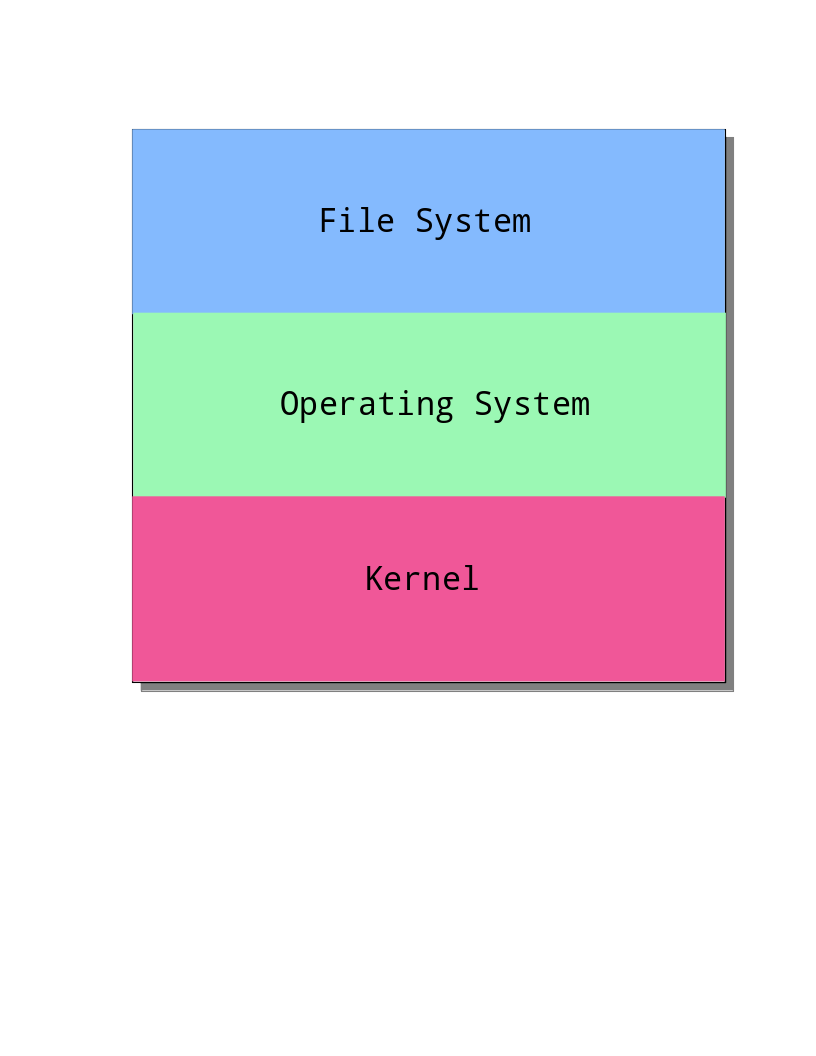
\includegraphics[width=0.5\textwidth]{media/images/comp-abstract.png}
    \end{wrapfigure}
	\begin{itemize}
		\item File System (FS)
		\item Operating System (OS)
		\item Kernel
	\end{itemize}


\end{frame}
\begin{frame}[fragile]{Extensions}

    There are several ways to augment a computer
    
    \begin{figure}
    \centering
    \begin{subfigure}{.5\textwidth}
        \centering
        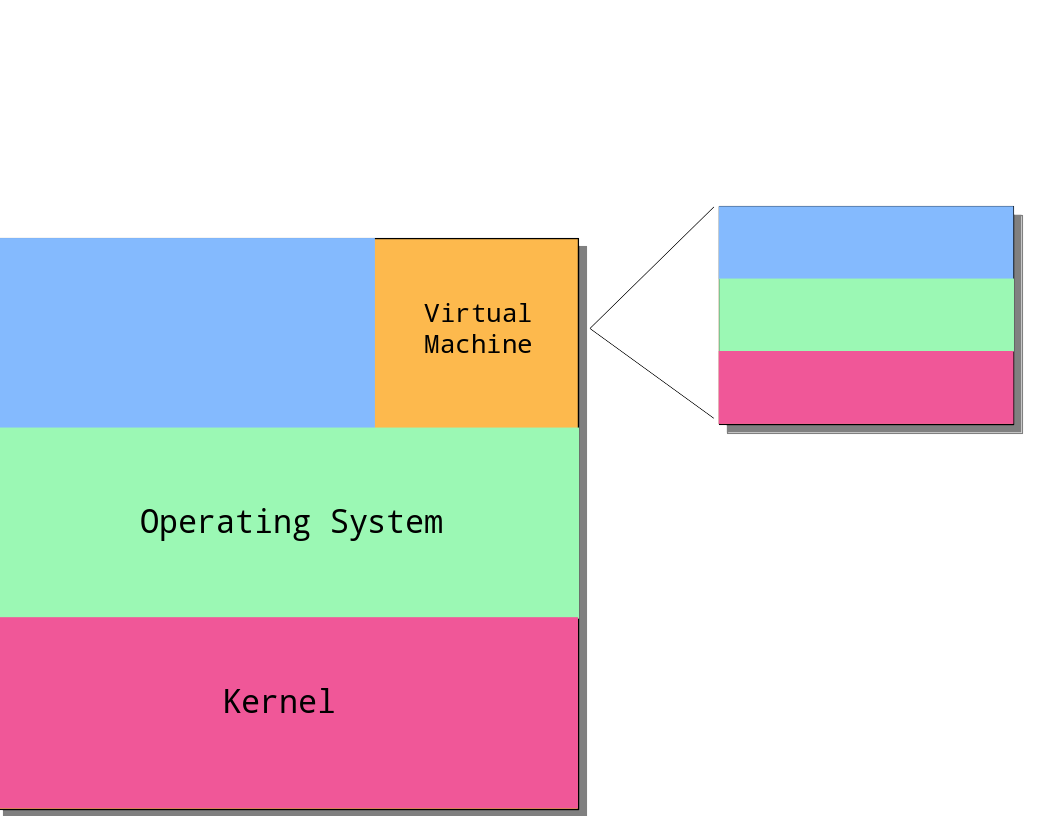
\includegraphics[width=0.9\textwidth]{media/images/comp-vm.png}
        \caption{Virtual Machine}
    \end{subfigure}%
    \begin{subfigure}{.5\textwidth}
        \centering
        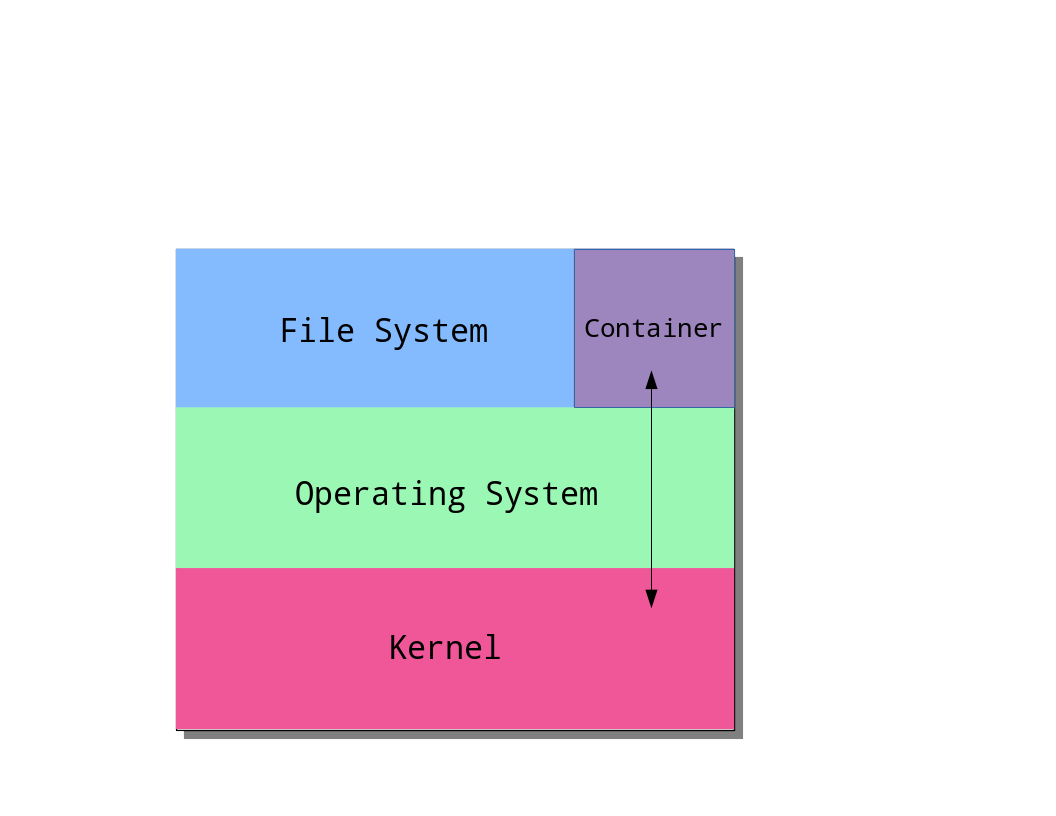
\includegraphics[width=0.9\textwidth]{media/images/comp-container.png}
        \caption{Container}
    \end{subfigure}
    \end{figure}
    

\end{frame}


\begin{frame}{Virtual Machines}
    
	\begin{figure}[l]
        \centering
        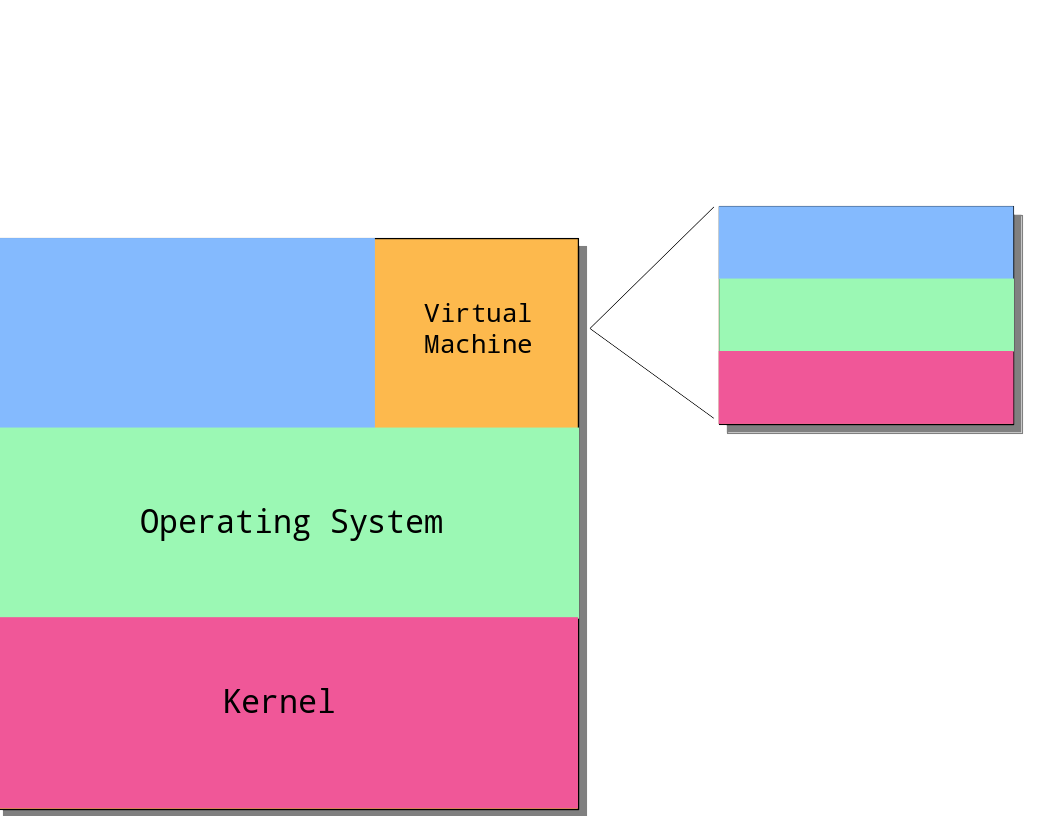
\includegraphics[width=0.5\textwidth]{media/images/comp-vm.png}
    \end{figure}
    Pros:
    \begin{itemize}
        \item Relatively universal (assuming OS and hardware support)
        \item Extensive configuration
    \end{itemize}
    Cons:
    \begin{itemize}
        \item Resource intensive
        \item Security concerns
    \end{itemize}
    
\end{frame}

\begin{frame}[fragile]{Containers}
    
	\begin{figure}[l]
        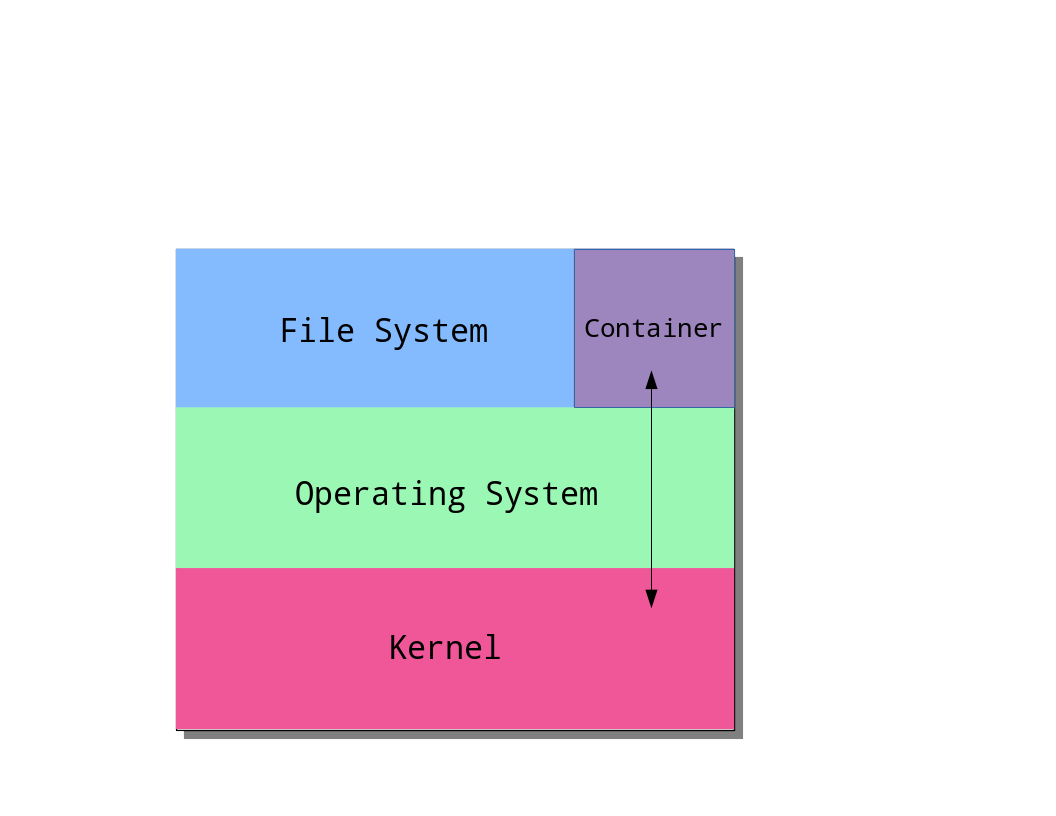
\includegraphics[width=0.5\textwidth]{media/images/comp-container.png}
    \end{figure}
    Pros:
    \begin{itemize}
        \item Low overhead
        \item Flexible deployment
    \end{itemize}
    Cons:
    \begin{itemize}
        \item Kernel limitations
    \end{itemize}
    
\end{frame}

\begin{frame}[fragile]{Container interactions with host}
    \begin{figure}[c]
    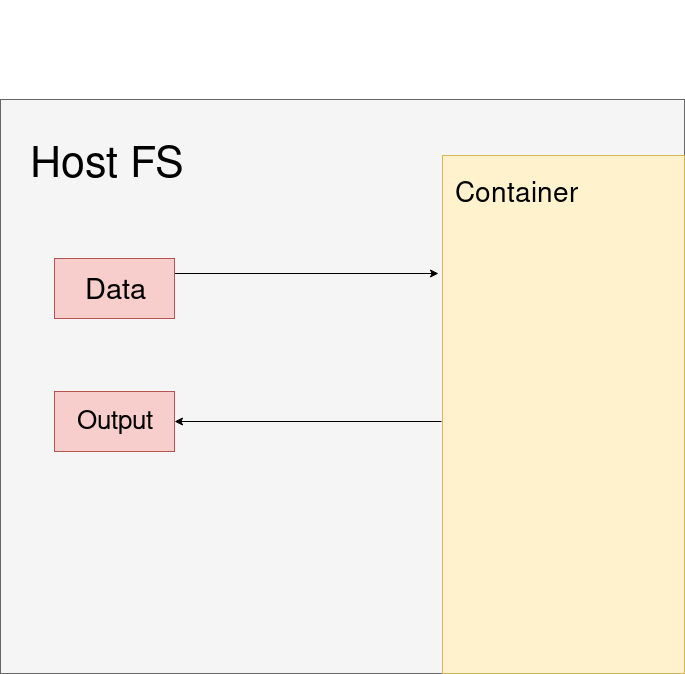
\includegraphics[scale=0.30]{media/images/workshop-diagrams-Host-concept-3-simple.png}
    \end{figure}
\end{frame}

\begin{frame}[fragile]{Container interactions with host}
    \begin{figure}[c]
    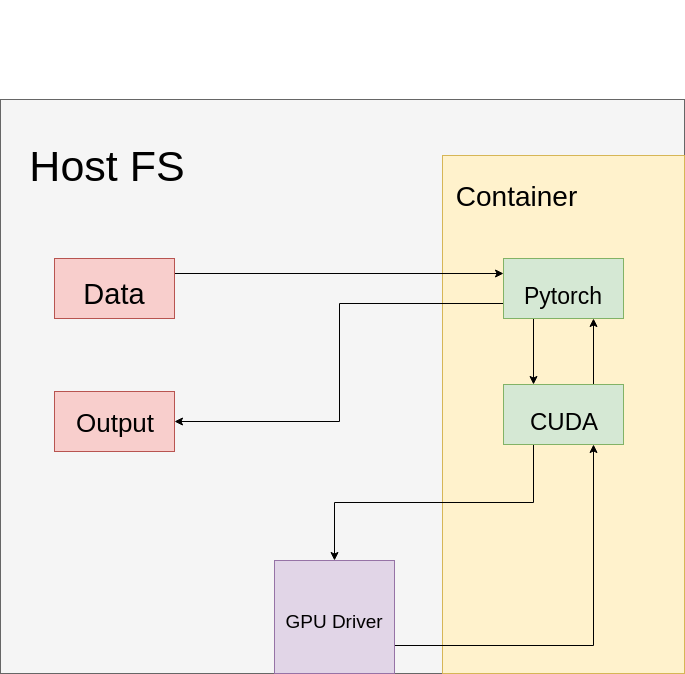
\includegraphics[scale=0.30]{media/images/workshop-diagrams-Host-concept-3.png}
    \end{figure}
\end{frame}

\section{Singularity: Getting Started}

\begin{frame}{Examples to follow along}
This presentation can be found here:\\
\url{https://github.com/CNCLgithub/singularity_workshop_2019}
\end{frame}

\begin{frame}[fragile]{Pulling containers}
    Containers can be pulled from container repos
    \begin{minted}
    [
    bgcolor=white,
    fontsize=\small
    ]
    {bash}
    # pulls from sylabs repos
    $ singularity pull alpine.sif library://alpine:latest
    # pulls from docker repos
    $ singularity pull tensorflow.sif \
    docker://tensorflow/tensorflow:latest
    \end{minted}
    
    These are immutable!
\end{frame}

\begin{frame}[fragile]{Building containers: Definition File}
    \scriptsize{\url{https://github.com/belledon/docker-singularity/blob/master/Singularity}}
    \noindent\makebox[\linewidth]{\rule{\paperwidth}{0.4pt}}
    %\inputminted[fontsize=\scriptsize]{bash}{examples/Singularity.fasttext}
\end{frame}
\begin{frame}[fragile]{Whats going on?}
    \begin{figure}[c]
    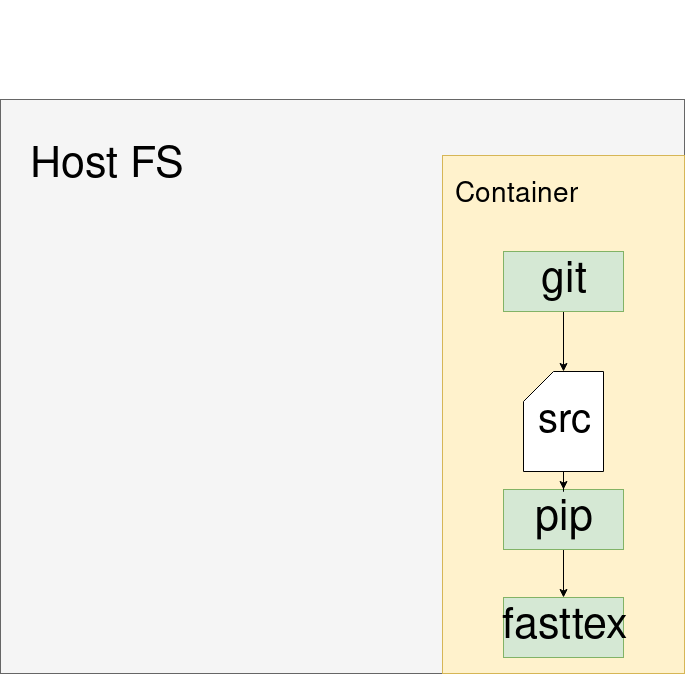
\includegraphics[scale=0.30]{media/images/workshop-diagrams-Host-concept-3-fasttext.png}
    \end{figure}
\end{frame}

\begin{frame}{Definition File components}
\begin{itemize}
    \item \texttt{\%post} - Run installation commands \textbf{after} setting up the parent
    \item \texttt{\%run} - Define the default executable behavior
    \item \texttt{\%environment} - Any env variables you would like defined
\end{itemize}
    
\end{frame}{}

\begin{frame}{Definition File components - extra}
\begin{itemize}
    \item \texttt{\%setup} - Any steps to run before running anything else
    \item \texttt{\%files} - Any files to copy to the host
    \item \texttt{\%help} - Describe the purpose of the container
\end{itemize}
    
    For more details please see the docs: \url{https://sylabs.io/guides/3.4/user-guide/definition_files.html}
\end{frame}{}

\begin{frame}{Don't reinvent the wheel!}
    You can often start from somewhere close!
    \noindent\makebox[\linewidth]{\rule{\paperwidth}{0.4pt}}
    % \inputminted[fontsize=\scriptsize]{bash}{examples/Singularity.julia}
\end{frame}

\begin{frame}{But don't be afraid}
    There will be times where you need to "take a step back"
    \noindent\makebox[\linewidth]{\rule{\paperwidth}{0.4pt}}
    % \inputminted[fontsize=\scriptsize]{bash}{examples/Singularity.pytorch-docker}

\end{frame}

\begin{frame}{Leaving the nest}
    For development, immutable containers aren't ideal
    \noindent\makebox[\linewidth]{\rule{\paperwidth}{0.4pt}}
    % \inputminted[fontsize=\scriptsize]{bash}{examples/Singularity.conda}
    
\end{frame}

\begin{frame}[fragile]{Package managers within containers}
	\begin{figure}[c]
        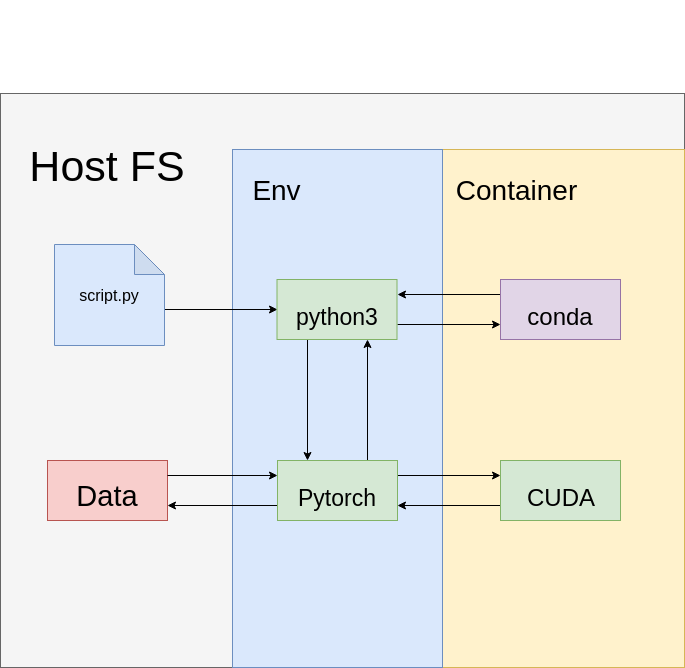
\includegraphics[scale=0.3]{media/images/workshop-diagrams-container-concept-package-manager.png}
    \end{figure}
\end{frame}

\section{Singularity: Using HPCs}

\begin{frame}{One module to rule them all}
\begin{itemize}
    \item A built container does not require sudo
    \item The container is one image file
    \item Ensures reproducibility 
\end{itemize}
\cite{Sing}
\end{frame}

\begin{frame}[fragile]{Getting your container on the HPC}
The simplest way to get started is to build a container on your local machine.

    \begin{minted}
    [
    bgcolor=white,
    fontsize=\small
    ]
    {bash}
    $ scp $CONT \
    > $USERNAME@<cluster>.yale.edu:/some/path

    \end{minted}

Alternatively, you could host your container online.
    \begin{minted}
    [
    bgcolor=white,
    fontsize=\small
    ]
    {bash}
    $ wget "http://www.my_cool_container/..."
    
    \end{minted}
\end{frame}

\begin{frame}{Building on HPC}
Not entirely reliable due to privileges. 

Typically done via vagrant and virtualbox

\end{frame}


\begin{frame}[fragile]{Running a container in a compute node}
    \begin{minted}
    [
    bgcolor=white,
    fontsize=\small
    ]
    {bash}
    $ cat my_sbatch.sh
    #!/bin/bash
    #SBATCH array=0-4
    #
    # note on Grace/milgram, singularity is available by 
    # default on compute nodes
    singularity exec ./train_nature_paper.sh
    
    \end{minted}    
\end{frame}


\begin{frame}{Problem: Modifying a container}
    Not possible on OM due to privileges.
    
    In most cases this is not necessary (keeping source and data outside of the container).
    
    However, there is an exception during development
\end{frame}




{\setbeamercolor{palette primary}{fg=black, bg=yellow}
\begin{frame}[standout]
  Extra slides on HPCs
\end{frame}
}

\appendix
\begin{frame}{Summary}

  Get the source of this theme and the demo presentation from

  \begin{center}\url{github.com/matze/mtheme}\end{center}

  The theme \emph{itself} is licensed under a
  \href{http://creativecommons.org/licenses/by-sa/4.0/}{Creative Commons
  Attribution-ShareAlike 4.0 International License}.

  \begin{center}\ccbysa\end{center}

\end{frame}

\section{Collaborative Documentation}

\begin{frame}{Useful linux commands}
    \begin{itemize}
        \item man
        \item ssh
        \item scp
        \item module
        \item awk
    \end{itemize}
\end{frame}

\section{High Performance Clusters}

\begin{frame}[fragile]{Interacting with an HPC}
    connecting to the head node
    \begin{minted}
    [bgcolor=white]
    {bash}
        ssh "${USERNAME}@openmind7.mit.edu"
    \end{minted}
	\begin{figure}[c]
        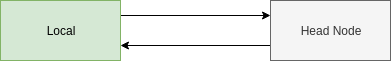
\includegraphics[width=0.75\textwidth]{media/images/workshop-diagrams-HPC-ssh-1.png}
    \end{figure}
\end{frame}

\note[itemize]{
\item To begin lets describe what happens when we want to talk to the HPC
\item SSH will describe a connection between your LOCAL machine and the HEADNODE
}

\begin{frame}[fragile]{HelloWorld!}
    Running our first command on the headnode.
    \begin{minted}
    [
    fontsize=\footnotesize,
    bgcolor=white
    ]
    {bash}
    $ whoami
    belledon
    \end{minted}
	\begin{figure}[c]
        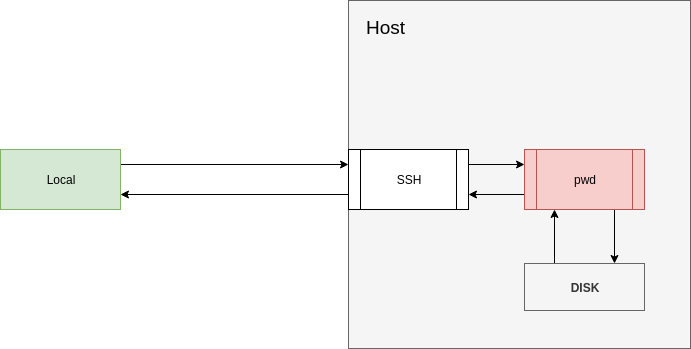
\includegraphics[scale=0.35]{media/images/workshop-diagrams-HPC-SSH-disk.png}
    \end{figure}
\end{frame}

\begin{frame}[fragile]{What is where?}
    Now that we know who we are, where are we?
    \begin{minted}
    [
    fontsize=\footnotesize,
    bgcolor=white
    ]
    {bash}
    $ pwd
    /home/$USER
    \end{minted}
	\begin{figure}[c]
        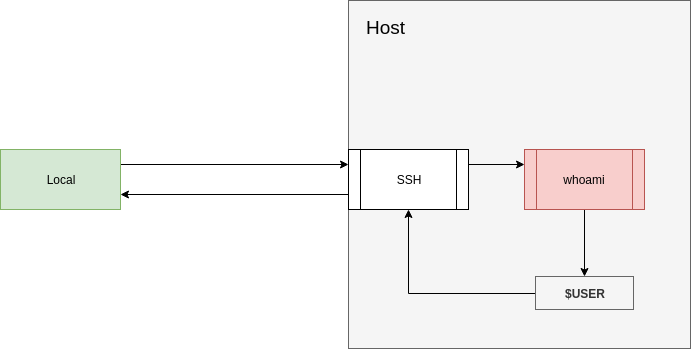
\includegraphics[scale=0.35]{media/images/workshop-diagrams-HPC-SSH-Helloworld.png}
    \end{figure}
\end{frame}


\begin{frame}[fragile]{Home is where the config is}
     
\$HOME should only be used for private configs, ssh-keys...
\begin{minted}
[
bgcolor=white,
fontsize=\footnotesize
]
{bash}
$ ls -alh ~/
total 216K
drwxr-xr-x   6 belledon tenenbaum   81 Jun 20 11:31 .cache
drwxr-xr-x  20 belledon tenenbaum 4.0K Oct 23  2018 .config
drwx------   2 belledon tenenbaum 4.0K Oct 12  2018 .ssh
-rw-r--r--   1 belledon tenenbaum  125 May 25  2017 rsync.sh
\end{minted}
\end{frame}

\begin{frame}{HPC Storage: Lustre}
\begin{itemize}
    \item Lustre file system supports fast, scalable IO \cite{Lustre}
    \item Sensitive to large number of files
    \item Resilient to the size of files
    \item Accessed via "/om"
\end{itemize}
\end{frame}

\begin{frame}{HPC Storage: NFS}
\begin{itemize}
    \item Supports basic network drives \cite{NFS}
    \item Sensitive to IO
    \item Resilient to the number of files
    \item Accessed via "/om2"
\end{itemize}

\end{frame}
\begin{frame}[fragile]{Accessing remote disks}
    
    \begin{minted}
    [
    bgcolor=white
    ]
    {bash}
        ls -l /om 
    \end{minted}
	\begin{figure}[c]
        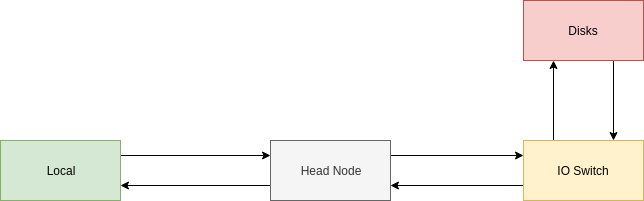
\includegraphics[width=\textwidth]{media/images/workshop-diagrams-HPC-ssh-2.png}
    \end{figure}
\end{frame}

\note[itemize]{
	\item Lets run the following command and describe what happens
    \item Normally
}

\begin{frame}[fragile]{Getting in Trouble}
    Finally... now lets get started
    \begin{minted}[bgcolor=white]{bash}
        ./train_nature_paper.sh 
    \end{minted}
\end{frame}

\begin{frame}[fragile]{Accessing resources}
    Requesting an interactive job
    \begin{minted}
    [
    fontsize=\footnotesize,
    bgcolor=white
    ]
    {bash}
    srun -c 4 --mem=8G --qos="$GROUP" -t 1-0 --pty bash
    \end{minted}
	\begin{figure}[c]
        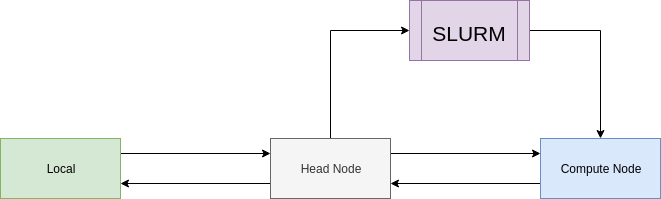
\includegraphics[width=\textwidth]{media/images/workshop-diagrams-SLURM-srun.png}
    \end{figure}
\end{frame}

\begin{frame}[fragile]{Accessing more resources}
    Requesting a batch job
    \begin{minted}
    [
    fontsize=\footnotesize,
    bgcolor=white
    ]
    {bash}
    $ cat example.sh
    #!/bin/bash
    #SBATCH --array=1-5
    echo "The array id is: ${SLURM_ARRAY_TASK_ID}"
    
    $ sbatch example.sh
    Submitted batch job 13873280 
    
    $ find . -name "*.out" | \
      while read src; do echo "${src} -> $(cat ${src})"; done
    ./slurm-13873280_5.out -> The array id is: 5
    ./slurm-13873280_2.out -> The array id is: 2
    ./slurm-13873280_3.out -> The array id is: 3
    ./slurm-13873280_1.out -> The array id is: 1
    ./slurm-13873280_4.out -> The array id is: 4 
    \end{minted}
\end{frame}


\begin{frame}[fragile]{Exploring SBATCH Tasks}
    \begin{figure}[c]
    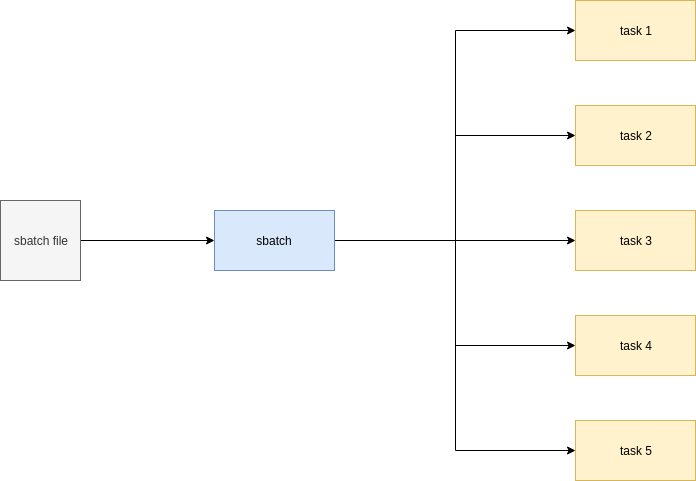
\includegraphics[scale=0.35]{media/images/workshop-diagrams-sbatch-1.png}
    \end{figure}
\end{frame}

\begin{frame}[fragile]{SBATCH Example: Hyperparameter search}
\begin{minted}
[
bgcolor = white,
fontsize=\footnotesize
]
{bash}
$ cat network_params.txt
--lr 0.0005
--lr 0.005
--lr 0.00005

$ cat my_sbatch.sh
#!/bin/bash
#SBATCH --time=1-0
#SBATCH --array=1-5
#SBATCH --gres=gpu:1
ARGUMENTS=$(sed "${SLURM_ARRAY_TASK_ID}q;d" network_params.txt)
./train_model "$ARGUMENTS"
\end{minted}
\end{frame}

\begin{frame}{SBATCH Example contd}
    \begin{figure}[c]
    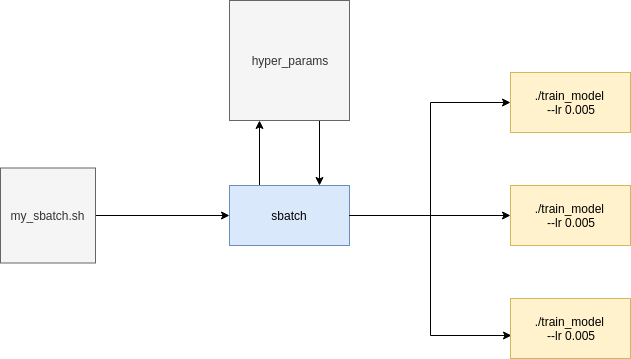
\includegraphics[scale=0.35]{media/images/workshop-diagrams-sbatch-2.png}
    \end{figure}
\end{frame}

\begin{frame}[fragile]{Adding project dependencies}

On many HPCs, managing software dependencies is done via "module". 

\begin{description}
    \mint{bash}|module avail| Shows modules you can add
    \mint{bash}|module add| Adds a module to your environment
    \mint{bash}|module list| Shows which modules you have
    \mint{bash}|module purge| Removes modules from environment
    
\end{description}
\end{frame}

\begin{frame}[fragile]{Adding a package}
This snippet adds "singularity" to my env
    \begin{minted}
    [
    bgcolor=white,
    fontsize=\small
    ]
    {bash}
    -bash-4.2$ module add openmind/singularity/3.2.0
    -bash-4.2$ singularity --version
    singularity version 3.2.0-1
    \end{minted}
\end{frame}

\begin{frame}{Problem: Computing environment}

\begin{itemize}
    \item Required module doesn't exist?
    \item Can't install dependency?
    \item Project environment behaves erratically?
\end{itemize}
    
\end{frame}


\begin{frame}[fragile]{HPCs, they're simple as 123}
    HPCs are to PCs as modern industrial economies are to aggrarian societies.
    \begin{description}
        \item Division of labour: 
        \begin{itemize}
            \item Compute
            \item IO
            \item Disk
        \end{itemize}
        \item Regulatory Trade Agencies
        \begin{itemize}
            \item Job Scheduling
            \item Service Monitoring
        \end{itemize}
        \item Chaos
        \begin{itemize}
            \item You (users)
            \item The man (admins)
            \item God (hardware failures)
        \end{itemize}
    \end{description}
\end{frame}
\begin{frame}[allowframebreaks]{References}

  \bibliography{main}
  \bibliographystyle{plain}

\end{frame}

\end{document}
